

IMU sensors are used in many driving analytics 
applications \cite{hansenspeed, wang2013sensing, chen2015invisible}. 
However, existing work assume the car is moving on flat 
roads and the smartphone is stably mounted in the vehicle. 
Different from these work, we propose several novel
techniques to improve the accuracy and usability of inertial sensors
by detecting orientation change, modeling stability,  
conducting slope-aware coordinate alignment and linear
acceleration estimation in a more practical manner. 
We design a slope-aware solutions to conduct 
coordinate alignment and track linear acceleration
by removing the gravity component dynamically from the aligned accelerometer readings. 
Second, we use clustering techniques to detect 
relative orientation changes. 
Third, we use moving variance to model the mounting
stability of the smartphone and evaluate sensing accruacy
based on mounting statiblity. 

\subsection{Slope-Aware Alignment}
\label{slopeaware}


\begin{figure}[!tbph]
\vspace{0.0cm}
\hspace{-0.5cm}
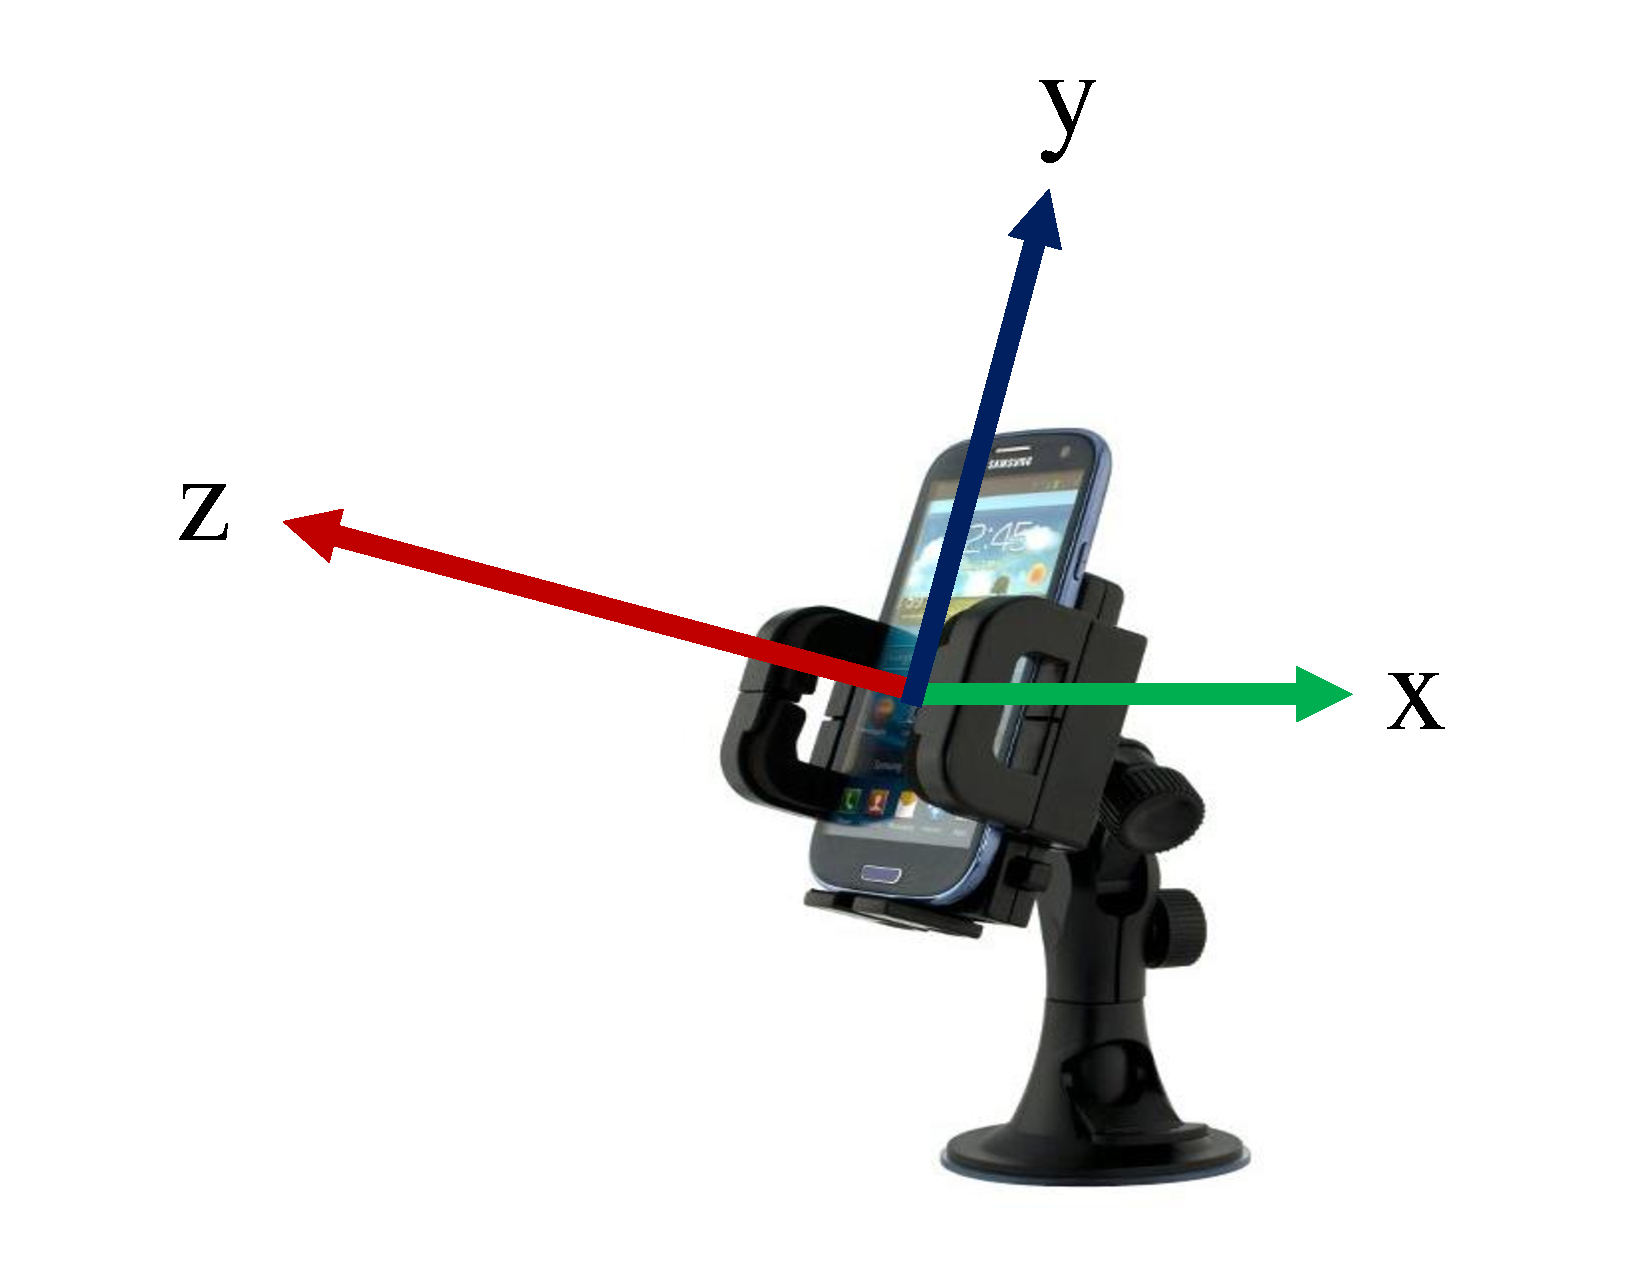
\includegraphics[width=1.8in,angle=0]{Figs/DriveSense/phone3d.pdf}
\vspace{0.0cm}
\hspace{-1.0cm}
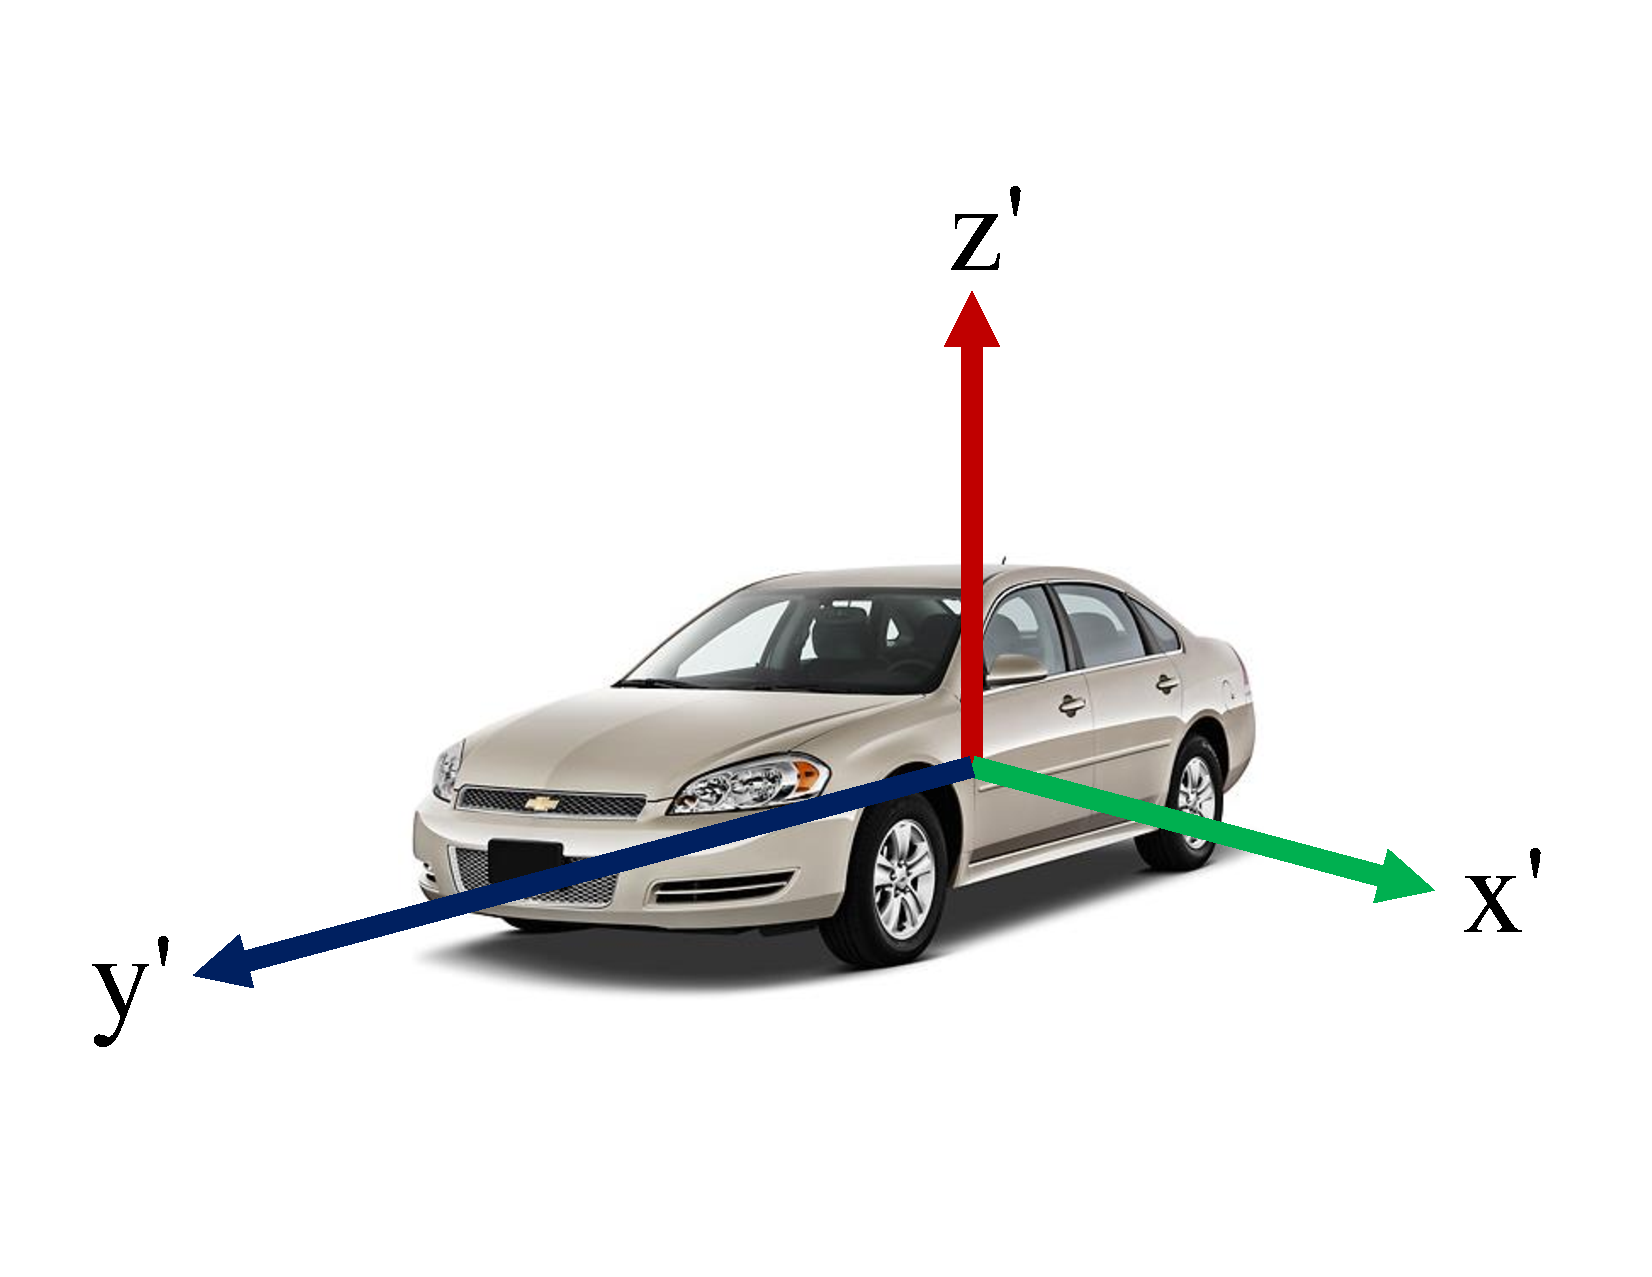
\includegraphics[width=1.8in,angle=0]{Figs/DriveSense/car3d.pdf}
\vspace{-0.2cm}
\caption{Coordinate system difference between a smartphone $[x, y, z]$ and a car $[x', y', z']$.}
\vspace{0.2cm}
\label{coordinates}
\end{figure}


\subsubsection{Slope-Aware Alignment and Linear Acceleration Estimation}


As illustrated in Fig. \ref{coordinates}, we use 
$[x, y, z]$ to represent the three dimensions of a smartphone
and use $[x', y', z']$ to represent the three dimensions
of a car. 
Coordinate alignment is the process that trains the rotation
matrix $R = [\hat{i}, \hat{j}, \hat{k}]$, 
where $\hat{i}$, $\hat{j}$ and $\hat{k}$ are three unit coordinate vectors,
so that $[x', y', z'] = [x, y, z] \times [\hat{i}, \hat{j}, \hat{k}]$.




\textbf{Step 1: Stop Points Extraction}. 

Identifying stop points are useful to conduct an initial alignment. 
We use a sliding window to track the deviation of the
accelerometer readings for this purpose.
The deviation is expected to be small when the car is stopped, 
i.e., in front of stop sign of red traffic light. 
But different cars have different vibrations, 
which affect the readings of the accelerometer. 
To identify a threshold for the deviation, 
we extract the stop points according to the speed information
collected from the OBD port.
We record the start time $s_t$ and end time $e_t$ that 
any speed reading in between is zero. 
To eliminate possible asynchronization and drifted value
after passing low-pass filter, 
we remove the points of the first 500ms and the last 500ms,
i.e., the data points within $[s_t + 500, e_t - 500]$. 
This process helps us to set the threshold to detect
stops. 
We only use OBD as a training input, 
our method can be used on any smartphone and vehicle settings
without OBD inputs. 
 

\textbf{Step 2: Horizontal Alignment}. 


Road slope affects the accuracy of coordinate alignment
in each step. 
During horizontal alignment, a slope-aware alignment method can
be much more effective than a slope-unaware approach. 
As illustrated in Fig. \ref{direction}, 
slope-unaware solutions assume all the data points 
pass the origin point and try to fit all the data
points for a single fit curve, 
while slope-aware solution treats each road segment
as different inputs (deviating from the origin point
due to slopes) and combine to improve the accuracy. 

To train the rotation matrix, we need to select the segments that the car is moving 
straight, and estimate the angle between the 
heading direction and the smartphone's horizontal coordinates \cite{wang2013sensing}.
To derive the rotation matrix from discrete sensor data points, 
we need to fit the curve and find the direction unit vector. 
We propose to train the horizontal
unit vector for each segment and combine each training results gradually with different weights.
There are lots of straight driving segments as illustrated in Fig. \ref{direction}, 
but not all of the segments are good for the training purpose. 
Each segment is selected based on the number of data points that
indicate the car is moving.
The intuition is that more data points could be more statistical significant. 
In Fig. \ref{direction}, we separate four segments and train the 
horizontal unit vector separately.
Clearly, this approach gives better view results that the four slopes of the 
fitting curves are $-0.98$, $-0.87$, $-0.93$ and $-0.95$, respectively. 
The weighted average is $-0.94$. 
After obtain the angle $a$, the horizontal 
rotation matrix can be calculated as follows. 

\[
R_h
	=
\begin{bmatrix}
   cos(\alpha) & -sin(\alpha) & 0 \\
   sin(\alpha) & cos(\alpha) & 0 \\
   0 & 0 & 1
\end{bmatrix}
\]



\begin{figure}[!tbph] 
\hspace{-0.4cm}
  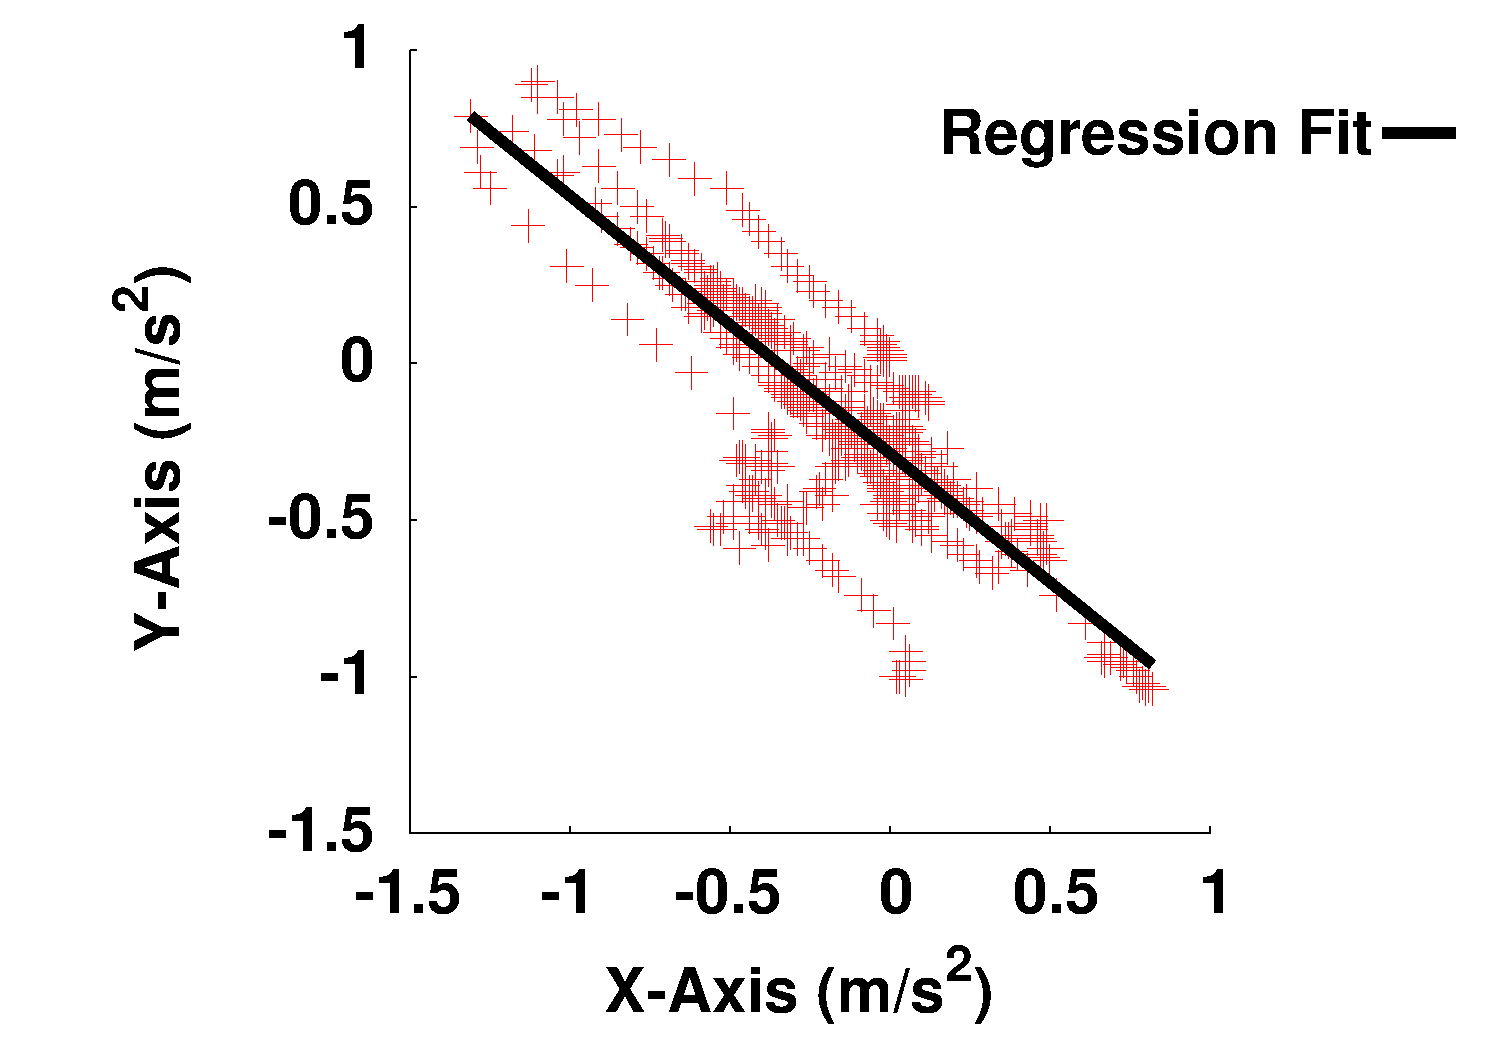
\includegraphics[width=2.6in,angle=0]{Figs/DriveSense/slopeaware/stateoftheart.pdf}
\hspace{-0.0cm}
  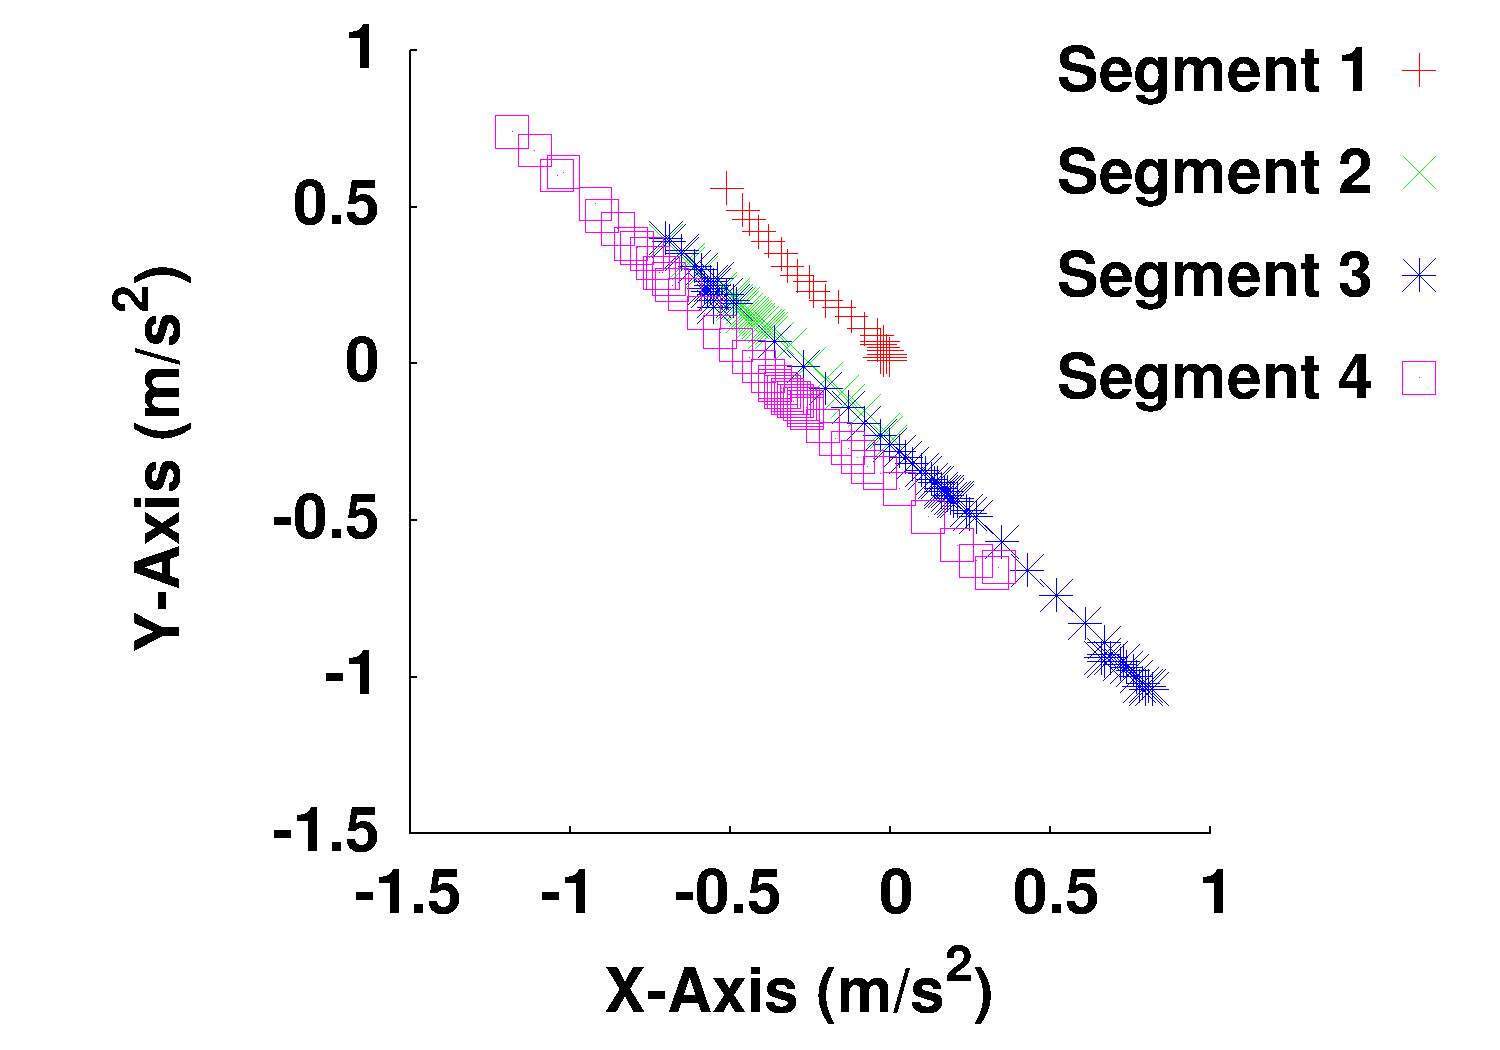
\includegraphics[width=2.6in,angle=0]{Figs/DriveSense/slopeaware/direction.pdf}
\hspace{-0.0cm}
   \caption{Training horizontal rotation matrix by using traditional
approach (above) and slope-aware multi-segment method (below).}
\label{direction}
\vspace{0.4cm}
\end{figure}





\begin{figure}[!htbp]
\begin{center}
%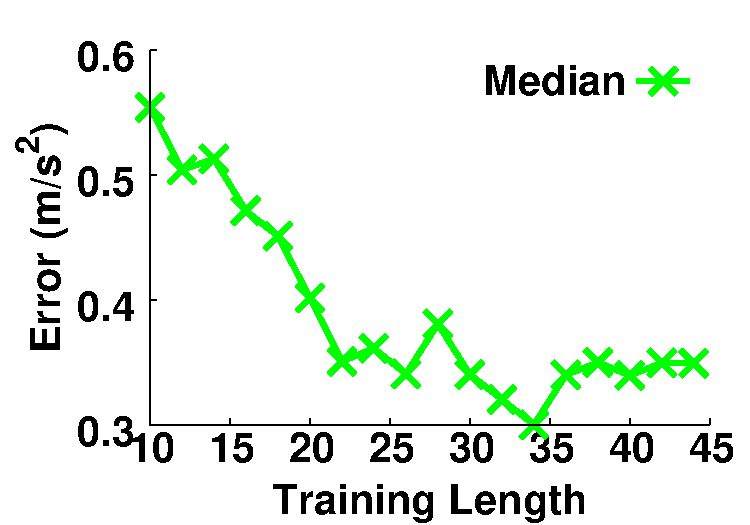
\includegraphics[width=1.7in,angle=0]{Figs/DriveSense/trainlengthanderror.pdf}
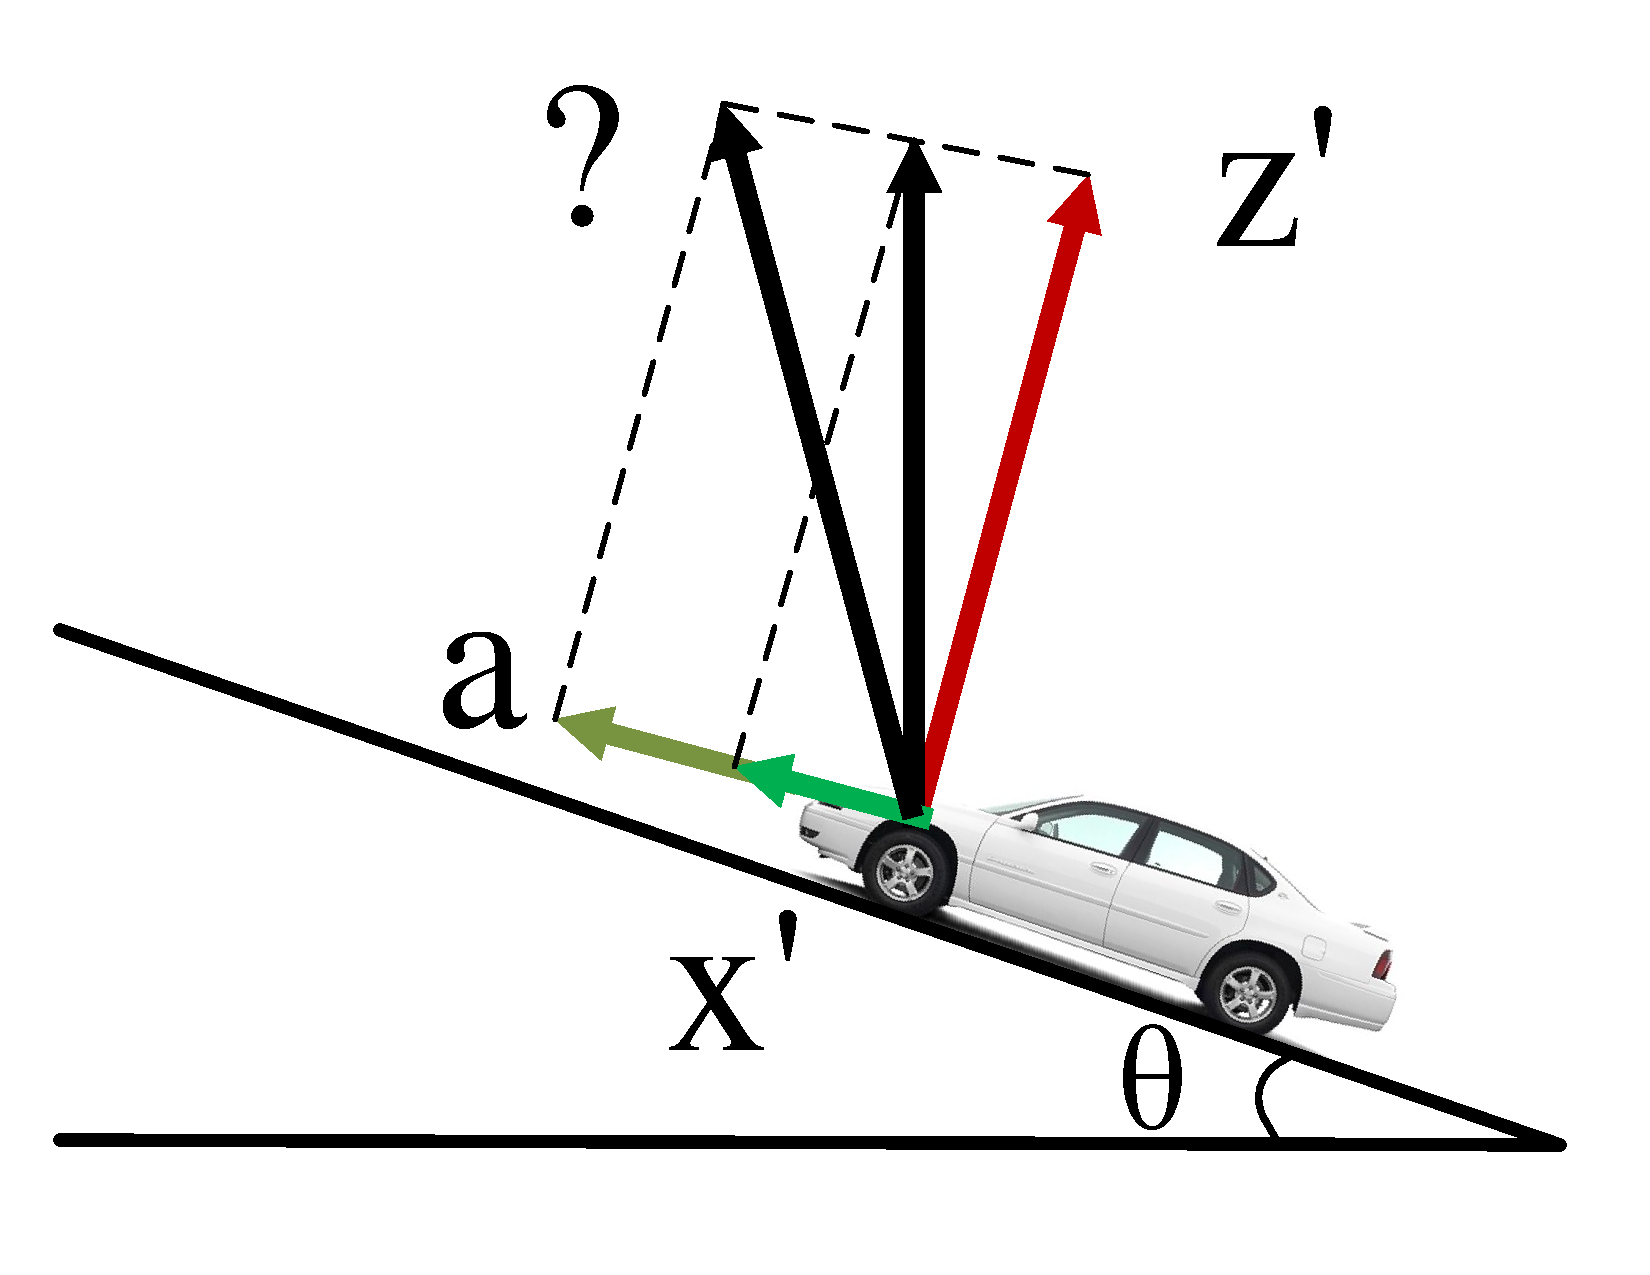
\includegraphics[width=2.0in, angle=0]{Figs/DriveSense/uncertain_vertical.pdf}
\vspace{0.0cm}
	\caption{
Since the actual acceleration of the car 
and the component of gravitational force (along the slope) are unknown, 
the direction of force is uncertain when conducting vertical alignment.
}
\label{training}
\vspace{0.4cm}
\end{center}
\end{figure}



\begin{algorithm}
\caption{Angle Search Algorithm}
\label{search}
\begin{algorithmic}[1]
\Input{$D_a$: The 2D accelerometer data after horizontal alignment}
\Output{$\theta_{o}$: The best fit angle}
\Procedure{AngleSearch}{}
\State $dev_{min} \gets MAX$;
\State $D_{t} \gets []$;
\For{$\theta$ \texttt{in} (-$\alpha$, $\alpha$)}
\For{$[y_i, z_i]$ \texttt{in} $D_a$}
\State $M_\nu$ $\gets$ $\begin{bmatrix}\cos\theta & -\sin\theta\ \\ \sin\theta & \cos\theta \end{bmatrix}$;
\State $[y'_i,z'_i]$ $\gets$ $[y_i,z_i]* M_\nu$;
\State $D_t.push(z'_i)$;
\EndFor
\State $dev_x \gets deviation(D_t)$;
\If {$dev_x < dev_{min}$}
\State {$dev_{min}$ $\gets$ $dev_x$};
\State {$\theta_{o}$ $\gets$ $\theta$};
\EndIf
\EndFor
\Return $\theta_{o}$;
\EndProcedure
\end{algorithmic}
\end{algorithm}
\vspace{-0.6cm}


\textbf{Step 3: Slope-Aware Alignment}. 

Estimating road slope at alignment time is challenging. 
In horizontal alignment, we can fit a curve as the moving
direction of the car (or the direction of force) is fixed and not much interfered 
by gravity. 
In vertical alignment, however, the direction of force is changing. 
As illustrated in Fig. \ref{training}, the direction of force changes
as the change of the acceleration of the car. 
There are two parameters are unknown, the slope gradient 
and the vehicle acceleration. 
The vehicle acceleration varies at each data point, 
which varies the direction of force and makes it is very
challenging to estimate the parameters.
We use one heuristic searching algorithm to search for best alignment angle. 
The algorithm relies on the property that the $z'-axis$ of 
the car should be constant over the same slope. 
Firstly, we assume the horizontal alignment is complete and
we convert a 3D alignment problem into a 2D alignment problem. 
The two dimensions are $y-axis$ and $z-axis$, 
as illustrated in Fig. \ref{training}.
By iterating over all the possible angles, 
we calculate deviation of the $z'-axis$ and locate the one with the least deviation. 
The pseudo code of the search algorithm is illustrated in 
Form \ref{search}.




\textbf{Step 4: Linear Acceleration Estimation}.



\begin{figure*}[t]
\begin{center}
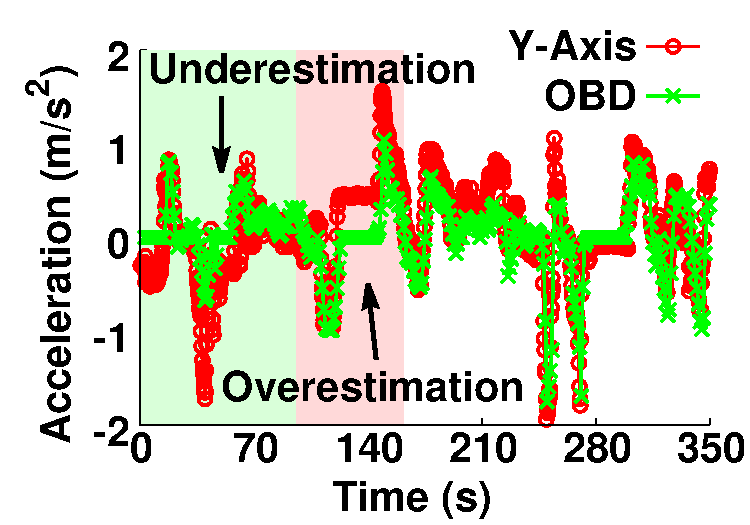
\includegraphics[width=2.2in,angle=0]{Figs/DriveSense/slopeaware/accspeed.pdf}
\hspace{-0.0cm}
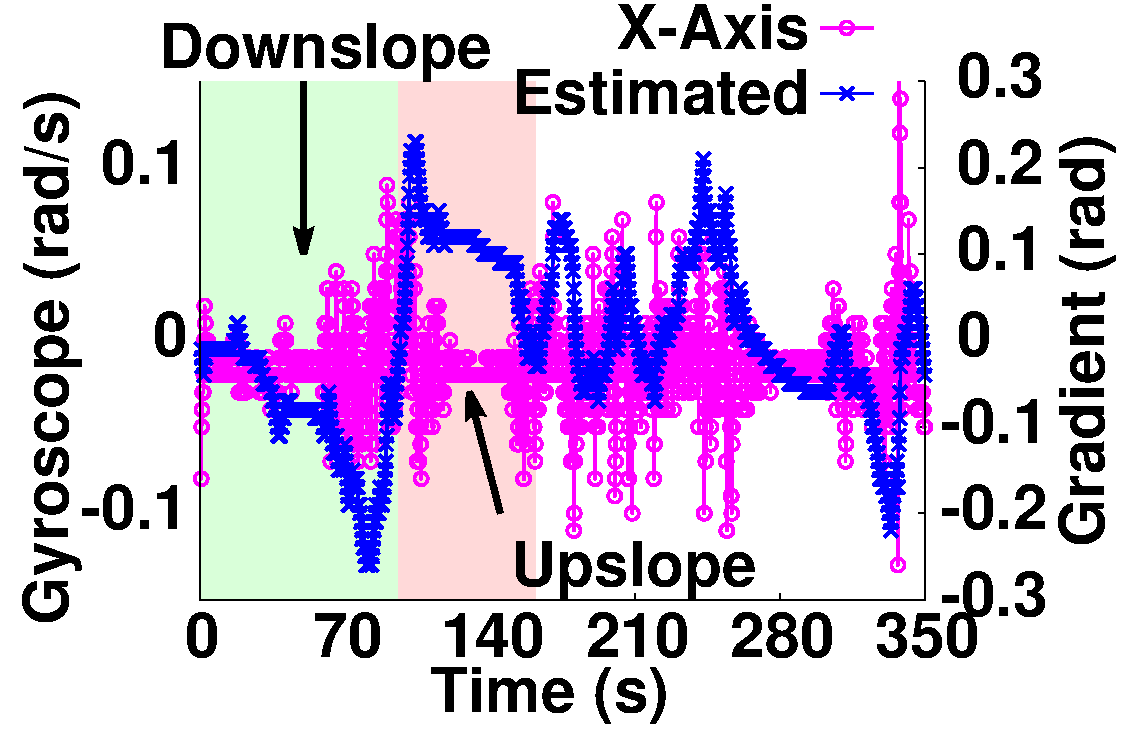
\includegraphics[width=2.2in,angle=0]{Figs/DriveSense/slopeaware/gyrocompare.pdf}
\hspace{-0.0cm}
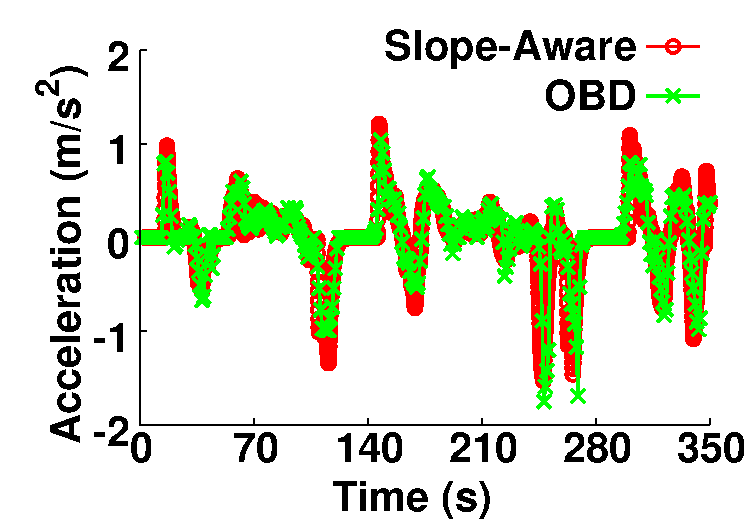
\includegraphics[width=2.2in,angle=0]{Figs/DriveSense/slopeaware/acccompare.pdf}
\hspace{-0.0cm}
\vspace{-0.2cm}
\caption{Slope-Aware coordinate alignment and linear acceleration estimation. 
The Figs/DriveSense are about acceleration over/under estimation caused by slopes (left), 
using gyroscope to estimate road slopes (middle), 
comparing estimated linear acceleration with groundtruth acceleration (right).}
\vspace{-0.2cm}
\label{linear_acceleration}
\end{center}
\end{figure*}


After coordinate alignment is complete, 
we can track the acceleration of a car by using the accelerometer's y-axis. 
We illustrate the acceleration values from aligned accelerometer 
in an example trip illustrated in Fig. \ref{linear_acceleration}. 
As the figure shows, comparing with the accelerations by OBD,   
the accelerations by the accelerometer of the first $90s$ 
are underestimated and the following $60s$ are overestimated.
This is because the car is moving mainly downslope and then mainly upslope. 
The deviated estimations may cause false positives/negatives on 
capturing driving behaviors such as brakes and accelerations.

We apply the same rotation matrix to the gyroscope data and 
illustrate the gyroscope x-axis data in Fig. \ref{linear_acceleration}.
After removing the constant drifts, 
it shows clear trends that the car is moving downslope and then
upslope.
Given the similar trends illustrated in two plots, 
we can estimate the slope gradient and deduct the gravitational force
components. 
We use similar calibration techniques proposed in \cite{zhou2014use}. 
We identify the road segments and stop points where accelerometer
can provide more accurate slope gradients to calibrate gyroscope.  



 

\subsection{Detecting Relative Orientation Change}


\begin{figure}[!htbp]
\begin{center}
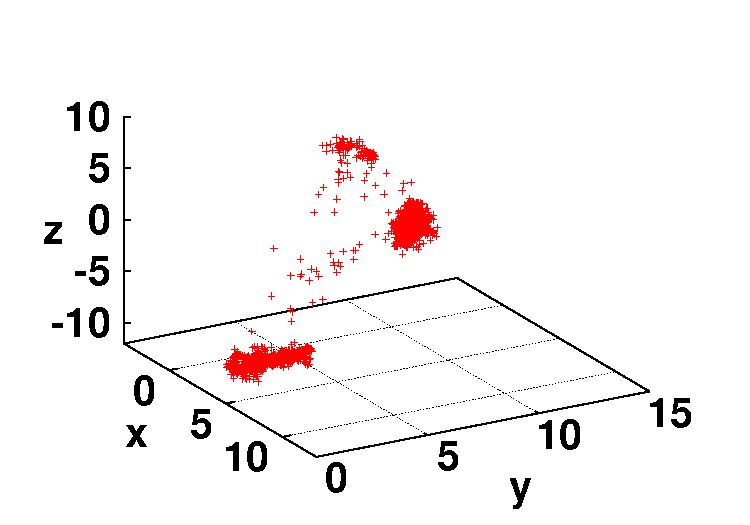
\includegraphics[width=1.7in,angle=0]{Figs/DriveSense/example_cluster.pdf}
\hspace{-0.8cm}
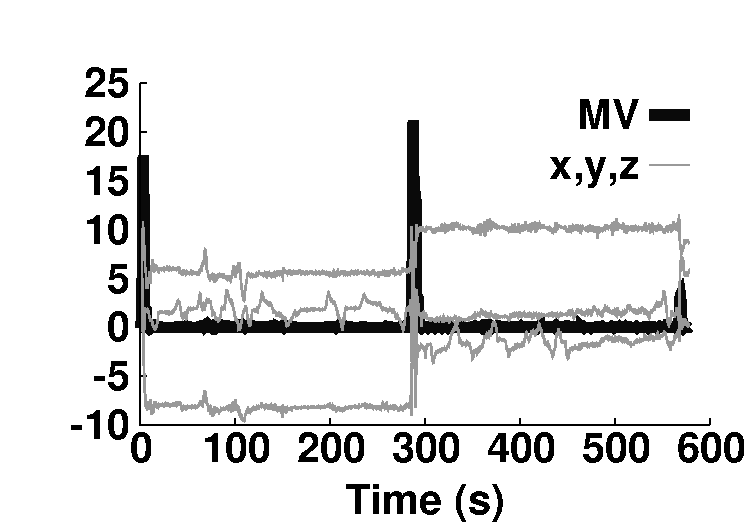
\includegraphics[width=1.7in,angle=0]{Figs/DriveSense/example_change.pdf}
\vspace{0.0cm}
\caption{The accelerometer data in one trip where the smartphone is picked up
from a pocket and put on the car mount holder. 
The upper cluster is formed when the user start the app at the beginning
and put the phone into the pocket, which is also detected by MV method. }
\vspace{-0.2cm}
\label{example_change}
\end{center}
\end{figure}


Using inertial sensors to estimate vehicle motions
is also vulnerable to smartphone relative orientation changes. 
Relative orientation refers to the relative orientation 
between the smartphone and the car.  
When the smartphone is fixed in the car and 
the car is moving upslope or making turns, the
relative orientation of the smartphone does not change 
as there is no relative movement between the smartphone
and the car.  
The relative orientation is usually changed by the smartphone
user, e.g., moving the smartphone from pocket to the car mount
for navigation.



The gyroscope is able to track absolute orientation changes
of the smartphone \cite{zhou2014use}. 
Tracking relative orientation change is a different. 
Since the smartphone is moving at the same pace 
with the car (suppose the smartphone is mounted), 
the gyroscope will sense the steering motions of the 
car, i.e., making turns, driving upslopes etc. 
It is challenging to separate the movement of the car
and the movement of the smartphone itself. 


We find accelerometer can be used to reliably detect orientation changes. 
While the movement of the car will introduce noises accelerometer
readings, but the noises are relatively small ($1-2m/s^2$ in most of the cases) 
in comparison to the gravitational force sensed by accelerometer. 
Once there is an orientation change, the gravity components
sensed by accelerometer are changed dramatically.
During one test trip, we move the smartphone
from pocket to car mount holder. 
The accelerometer sensor readings are illustrated in Fig. \ref{example_change}. 
All the accelerometer sensor readings can be naturally
classified into three clusters. 
The upper small one is formed when the user hold
the smartphone and manually start the app. 
The rest two are formed when the smartphone is in 
the pocket and on the car mount holder, respectively. 
Intuitively, incremental clustering methods are reasonable 
choices to identify orientation change, 
i.e., there is new cluster formed. 


\textbf{Incremental Clustering}. Traditional incremental clustering methods can be used in 
orientation change detection, e.g., 
orientation change happens when there is another cluster
emerges. 
The existing clustering methods are reliable enough
and tested by many applications 
\cite{nguyen2015survey, ordonez2003clustering, rodrigues2008hierarchical, song2005highly}. 
We test several common incremental clustering methods 
such as Sequential K-means (S-KM), Hierarchical Clustering (HCA) 
and Gaussian Mixture Models (GMM). 
The drawback of such approaches is the delay for detecting
another cluster, i.e., it requires enough data samples
to form a new cluster. 
In some real time applications such as brake warnings, 
false warning may happen if orientation change
is not detected in the first place. 
Due to the space limit, We refer interested 
readers to \cite{nguyen2015survey} for 
detailed descriptions of different methods.


\textbf{Moving Variance (MV)}. To timely detect orientation change before
another cluster is formed, 
we look at the change of a moving window.
The moving window contains $m$ data samples, 
and we use the variance of the moving window to detect
orientation changes. 
The intuition behind is that the changes of sensed gravity components 
is much more significant than those of caused by vehicle's movements. 
The variance can be calculated as $Var(x) = E[(X - \mu)^2]$, 
where $X$ is the euclidean distance to the ``moving cluster''
center and $\mu$ is the average distance. 
There are cases that the movement is too small to be detected
by MV. 
For example, a small horizontal rotation of the smartphone will not 
change the variance. 
We use the stability model to estimate such small changes. 
We will show in the later section that such looseness
make the acceleration estimation inaccurate. 
 
 
\subsection{Estimating Mounting Stability}



\begin{figure}[!htbp]
\begin{center}
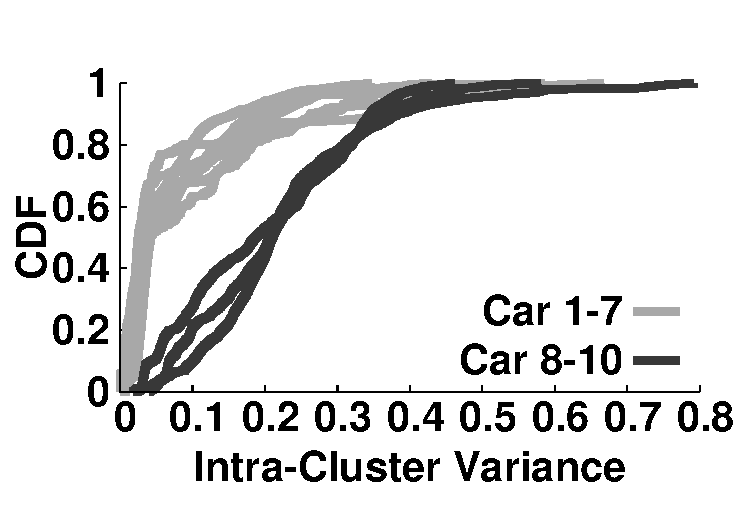
\includegraphics[width=1.7in,angle=0]{Figs/DriveSense/variance_cars.pdf}
\hspace{-0.5cm}
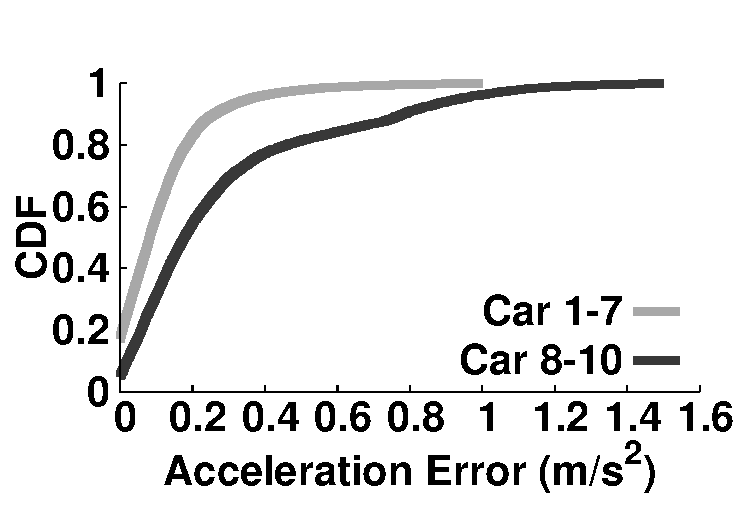
\includegraphics[width=1.7in,angle=0]{Figs/DriveSense/sensor_error_cars.pdf}
\vspace{-0.2cm}
\caption{The intra-cluster variance distribution of the tight group (car 1-7)
	and the loose group (car 8-10), and 
the estimated acceleration accuracy of the tight group is higher than those
	of the loose group.}
\vspace{-0.2cm}
\label{mounting}
\end{center}
\end{figure}


Another factor affects the accuracy of vehicle motion sensing
is the mounting stability of the smartphone. 
The stability of the smartphone depends on how the 
smartphone is fixed/placed/held in the car. 
A good case scenario is the user placing the smartphone
on a stable car mount holder. 
A bad case scenario is the user or passenger playing
motion games such as car racing which requires rotating
the smartphone. 
The derived sensor readings of the car are over noisy
due to shaking and/or rotating of the smartphone. 


We model one fixed relative orientation as a cluster of 
sensor readings. 
We use \emph{intra-cluster variance (ICV)} to estimate 
the stability of the smartphone.  
A stable mounting of the smartphone is expected to produce a smaller
variance than unstable holding by hands.  
Since ICV is correlated with the cluster
size, we use the ICV of the subclusters to represent
the ICV of the whole cluster. 
We define one subcluster is any continous $n$ 
points of the whole cluster.  
We use ICV to evaluate the mounting
stability of the tablets from dataset $\#1$. 
We firstly remove all the trips that there is orientation 
change detected. 
As shown in Fig. \ref{mounting}, 
all the data from the 10 cars are naturally divided into two groups, 
where the first group (car 1-7) has a median variance less than 0.05
and the second group (car 8-10) has a median variance around 0.2.
We name the first group as \emph{tight group} and 
the second one as \emph{loose group}. 
Since the tablets are not aligned with the cars, 
we conduct coordinate alignment and linear acceleration
estimation by using the methods in Section \ref{slopeaware}. 
We compare the acceleration estimated by aligned accelerometer
and the groundtruth acceleration calculated by OBD speed. 
As indicated in Fig. \ref{mounting}, 
the estimated accuracy of the tight group is generally higher
than the loose group. 


  


